\chapter{It\^o's Formula}\label{chap16}

\noindent
{\bf Motivation.}~ Let\pageoriginale $\beta(t)$ be a one-dimensional
Brownian motion. We have seen that the left integral
\begin{equation*}
L\left[2\int\limits^{t}_{0}\beta(s,\cdot)d\beta\right]=[\beta^{2}(t,\cdot)-\beta^{2}(0,\cdot)-t]\tag{*}
\end{equation*}

Formally (*) can be written as
$$
d\beta^{2}(t)=2\beta(t)d\beta(t)+dt.
$$

For, on integrating we recover (*).

Newtonian calculus gives the result:
$$
df(\beta(t))=f'(\beta(t))d\beta(t)+\frac{1}{2}f''(\beta(t))d\beta^{2}(t)+\cdots 
$$
for reasonably smooth functions $f$ and $\beta$. If $\beta$ is of
bounded variation, only the first term contributes something if we
integrate the above equation. This is because $\sum d\beta^{2}=0$ for
a function of bounded variation. For the Brownian motion we have seen
that $\sum d\beta^{2}\to$ a non zero value, but one can prove that
$\sum d\beta^{3},\ldots$ converge to $0$. We therefore expect the
following result to hold:
$$
df(\beta(t))\approx
f'(\beta(t))d\beta(t)+\frac{1}{2}f''(\beta(t))d^{2}\beta(t). 
$$

We show that for a one-dimensional Brownian motion
$$
\sum (d\beta)^{3},\q \sup(d\beta)^{4},\ldots
$$ 
all vanish.
\begin{figure}[H]
\centering
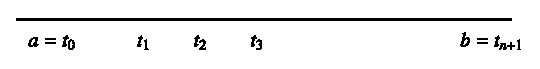
\includegraphics{figure/fig12.eps}
\end{figure}

\begin{gather*}
E(\sum(d\beta)^{3})=E\left(\sum\limits^{n}_{i=0}[\beta(t_{i+1})-\beta(t_{i})]^{3}\right)=\sum\limits_{i=0}E[(\beta(t_{i+1})-\beta(t_{i})]^{3}\\
=\sum^{n}_{i=1}0=0,
\end{gather*}\pageoriginale
because $\beta(t_{i+1})-\beta(t_{i})$ is a normal random variable with
mean zero and variance $t_{i+1}-t_{i}$. Similarly the higher odd
moments vanish. Even moments of a normal random variable with mean $0$
and variance $\sigma^{2}$ are connected by the formula
$$
\mu_{2k+2}=\sigma^{2}(2k+1)\mu_{2k},k>1.
$$

So
$$
\sum(d\beta)^{4}=\sum^{n}_{i=0}(\beta(t_{i+1})-\beta(t_{i}))^{4}.
$$

Therefore
\begin{align*}
E(\sum(d\beta)^{4}) &=
\sum^{n}_{i=0}E([\beta(t_{i+1})-\beta(t_{i}))^{4}]\\
&= 3\sum^{n}_{i=0}(t_{i+1}-t_{i})^{2};
\end{align*}
the right hand side converges to $0$ as the mesh of the partition goes
to $0$. Similarly the higher order even moments vanish.

More generally, if $\beta(t,\cdot)$ is a $d$-dimensional Brownian
motion then we expect
$$
df(\beta(t))\approx \nabla f(\beta(t))\cdot
d\beta(t)+\frac{1}{2}\sum_{i,j}\frac{\p^{2}f}{\p x_{i}\p
  x_{j}}d\beta_{i}d\beta_{j}.
$$

However $\sum d\beta_{i}d\beta_{j}=0$ if $i\neq j$ (see exercise
below). Therefore 
$$
df(\beta(t))\approx \nabla f(\beta(t))\cdot
d\beta(t)+\frac{1}{2}\Delta f(\beta(t))d\beta^{2}(t).
$$

The appearance of $\Delta$ on the right side above is related to the
heat equation.

\setcounter{exercise}{3}
\begin{exercise}\label{chap16-exer4}
Check\pageoriginale that $d\beta_{i}d\beta_{j}=\delta_{ij}dt$.

\noindent
(Hint: For $i=j$, the result was proved earlier. If $i\neq j$,
consider a partition $0=t_{0}<t_{1}<\ldots<t_{n}=t$. Let
$\Delta_{k}\beta_{i}=\beta_{i}(t_{k})-\beta_{i}(t_{k-1})$. Then
$$
E\left(\sum\limits^{n}_{k=1}\Delta_{k}\beta_{i}\Delta_{k}\beta_{j}\right)^{2}=\sum_{k}E(\Delta^{2}_{k}\beta_{i}\Delta^{2}_{k}\beta_{j})+2\sum\limits_{k\neq
  l}E[(\Delta_{k}\beta_{i})(\Delta_{1}\beta_{j})]; 
$$
the right side converges to $0$ as $n\to \infty$ because
$\Delta_{k}\beta_{i}$ and $\Delta_{\ell}\beta_{j}$ are independent for
$k\neq \ell$).

Before stating It\^o's formula, we prove a few preliminary results.
\end{exercise}

\setcounter{lemma}{0}
\begin{lemma}\label{chap16-lem1}
Let $X(t,\cdot)\in I[b,0]$ be a one-dimensional It\^o process. Then
$$
X(t,\cdot)-X(0,\cdot)=\int\limits^{t}_{0}b(s,\cdot)ds\q \text{a.e.}
$$
\end{lemma}

\begin{proof}
$\exp[\theta X(t,\cdot)-\theta
    X(0,\cdot)-\theta\int\limits^{t}_{0}b(s,\cdot)ds]$ is a martingale
  for each $\theta$. Therefore
$$
E(\exp[\theta(X(t,\cdot)-X(0,\cdot))-\theta\int\limits^{t}_{0}b(s,\cdot)ds])=\text{~constant~}=1,\ \forall t.
$$

Let 
$$
W(t,\cdot)=X(t,\cdot)-X(0,\cdot)-\int\limits^{t}_{0}b(s,\cdot)ds.
$$

Then 
$$
E(\exp \theta W(t,\cdot))=\text{~ Moment generating function of~ }
w=1,\ \forall t.
$$

Therefore $\theta(t,\cdot)=0$ a.e.
\end{proof}

\begin{remark*}
If\pageoriginale $X(t,\cdot)\in I[0,0]$ then $X(t,\cdot)=X(0,\cdot)$
a.e.; i.e.\@ 
$X(t,\cdot)$ is a trivial process.
\end{remark*}

We now state a theorem, which is a particular case of the theorem on
page \ref{page103}.


\begin{theorem*}
If $h\in C^{1,2}([0,\infty)\times \mathbb{R}^{d})$ such that {\rm(i)}
  $|h(x)|\leq A|x|+B$, $\forall x \in[0,\infty)\times
    \mathbb{R}^{d}$, for constants $A$ and $B$ {\rm(ii)} $\dfrac{\p
      h}{\p t}$, $\dfrac{\p h}{\p x_{i}}$, $\dfrac{\p^{2}h}{\p x_{i}\p
      x_{j}}$ also grow linearly, then
$$
\exp[h(t,\beta(t,\cdot)-\int\limits^{t}_{0}\left(\frac{\p h}{\p
    s}+\frac{1}{2}\Delta
  h\right)(s,\beta(s,\cdot)-\frac{1}{2}\int\limits^{t}_{0}|\nabla h|^{2}(s,\beta(s,\cdot))ds]
$$ 
is a martingale.
\end{theorem*}

\noindent
{\bf Ito's Formula.}~ Let $f\in C^{1,2}_{0}([0,\infty)\times
  \mathbb{R}^{d})$ and let $\beta(t,\cdot)$ be a $d$-dimensio\-nal
  Brownian motion. Then
\begin{align*}
& f(t,\beta(t))-f(0,\beta(0))=\int\limits^{t}_{0}\frac{\p f}{\p
  s}(s,\beta(s,\cdot))ds+\\
&\qq +\int\limits^{t}_{0}\langle \nabla
  f(s,\beta(s,\cdot)),d\beta(s,\cdot)\rangle
  +\frac{1}{2}\int\limits^{t}_{0}\Delta f(s,\beta(s,\cdot))ds.
\end{align*}
where
$$
\Delta\equiv \dfrac{\p^{2}}{\p x^{2}_{1}}+\cdots+\frac{\p^{2}}{\p
  x^{2}_{d}}.
$$

\begin{proof}

\setcounter{step}{0}
\begin{step}%1
Consider a $(d+1)$-dimensional process defined by
\begin{align*}
& X_{0}(t,\cdot)=f(t,\beta(t,\cdot)),\\
& X_{j}(t,\cdot)=\beta_{j}(t,\cdot).
\end{align*}

We claim that $X(t,\cdot)\equiv (X_{0},X_{1},\ldots,X_{d})$ is a
$(d+1)$-dimensional It\^o-process with parameters
$$
b=\left[\left(\frac{\p f}{\p s}+\frac{1}{2}\Delta
  f\right)(s,\beta(s,\cdot)),0,0,\ldots 0\right]\q d\text{~ terms}
$$
and\pageoriginale
$$
a=
\begin{bmatrix}
a_{00} & a_{01} & \ldots & a_{0d}\\
a_{10} & & & \\
\ddots & & & I_{d\times d}\\
a_{d0} & & & 
\end{bmatrix}
$$
where 
\begin{align*}
a_{00} &= |\nabla_{x}f|^{2}(s,\beta(s,\cdot)),\\
a_{0j} &= \left(\frac{\p}{\p x_{j}}f\right)(s,\beta(s,\cdot)),\\
a_{j0} &= a_{0j}.
\end{align*}

For, put $h=\lambda f(t,x)+\langle \theta, x\rangle$,
$x=(x_{1},\ldots,x_{d})\in \mathbb{R}^{d}$, in the previous
theorem. Then
$$
\frac{\p h}{\p s}=\lambda\frac{\p f}{\p s},\Delta h=\lambda\Delta
f,\frac{\p h}{\p x_{j}}=\lambda\frac{\p f}{\p x_{j}}+\theta_{j}. 
$$
Therefore we seen that
\begin{align*}
&\exp[\lambda f(t,\beta(t,\cdot))+\langle
  \theta,\beta(t,\cdot)\rangle-\lambda\int\limits^{t}_{0}\left(\frac{\p
    f}{\p s}+\frac{1}{2}\Delta_{x}f\right)(s,\beta(s,\cdot)ds\\
&-\frac{1}{2}\lambda^{2}\int\limits^{t}_{0}|\nabla
  f|^{2}(s,\beta(s,\cdot))ds-\frac{1}{2}|\theta|^{2}t-\lambda\langle\theta,\int\limits^{t}_{0}\nabla (f(s,\beta(s,\cdot)))ds\rangle]
\end{align*}
is a martingale.

Consider $(\lambda,\theta)a\binom{\lambda}{\theta}$. We have
$$
a
\begin{bmatrix}
\lambda\\
\theta
\end{bmatrix}
=
\begin{bmatrix}
a_{00}\lambda +\sum^{d}_{j=1}a_{0j}\theta_{j}\\
\rho+\theta
\end{bmatrix}
,\q \rho=\lambda
\begin{bmatrix}
a_{10}\\
\ddots\\
a_{d0}
\end{bmatrix}.
$$

Therefore
\begin{align*}
(\lambda,\theta)a
\begin{bmatrix}
\lambda\\
\theta
\end{bmatrix}
&=
a_{00}\lambda^{2}+\lambda\sum\limits^{d}_{j=1}a_{0j}\theta_{j}+\sum\limits^{d}_{j=1}a_{0j}\theta_{j}+\\
&= \lambda^{2}|\nabla f|^{2}+2\lambda \frac{\p f}{\p
  x_{j}}\theta_{j}+|\theta|^{2}. 
\end{align*}\pageoriginale

Thus (*) reads
$$
\exp[\lambda
  f(t,\beta(t,\cdot)+\langle\theta,\beta(t,\cdot)\rangle-\lambda\int\limits^{t}_{0}b_{0}(s,\cdot)ds-\frac{1}{2}\int\limits^{t}_{0}\langle
  \alpha,a\alpha\rangle ds]
$$
is a martingale where $\alpha=(\lambda,\theta)\in
\mathbb{R}^{d+1}$. This proves the claim made above.
\end{step}

\begin{step}%2
Derine $\sigma(s,\cdot)=(1,-\nabla_{x}f(s,\beta(s,\cdot)))$ and let
$$
Z(t,\cdot)=\int\limits^{t}_{0}\langle
\sigma(s,\cdot),dX(s,\cdot)\rangle\text{~ where~ } X\approx
(X_{0},X_{1},\ldots,X_{d}) 
$$
is the $(d+1)$-dimensional It\^o process obtained in Step 1. Since
$f\in C^{1,2}_{b}$, $Z(t,\cdot)$ is an It\^o process with parameters
$\langle \sigma,b\rangle$ and $\sigma a\sigma^{*}$:
\begin{align*}
\langle \sigma,b\rangle &= \frac{\p f}{\p s}+\frac{1}{2}\Delta f,\\
a\sigma^{*} &= 
\begin{bmatrix}
a_{00} & \rho\\
\rho^{*} & I
\end{bmatrix}
\begin{bmatrix}
1\\
-\nabla_{x}f
\end{bmatrix}\\
&= 
\begin{bmatrix}
a_{00}-\langle \rho,\nabla_{x}f\rangle\\
\rho^{*}-\nabla_{x}f
\end{bmatrix}
=
\begin{bmatrix}
0\\
0\\
\vdots\\
0
\end{bmatrix}
\end{align*}

Therefore $\sigma a\sigma^{*}=0$. Hence by Lemma \ref{chap16-lem1},
$$
Z(t,\cdot)-Z(0,\cdot)-\int\limits^{t}_{0}\langle \sigma,b\rangle
ds=0\text{(a.e.)}, 
$$
\begin{align*}
Z(t,\cdot) &= \int\limits^{t}_{0}dX_{0}(s)-\int\limits^{t}_{0}\langle
\nabla f(s,\beta(s,\cdot)),d\beta(s,\cdot)\rangle\\
&= f(t,\beta(t))-f(0,\beta(0))-\int\limits^{t}_{0}\langle \nabla f(f,\beta(s,\cdot)),d\beta(s,\cdot)\rangle
\end{align*}\pageoriginale

Hence $Z(0)=0$. Thus
\begin{align*}
f(t,\beta(t)) &- f(0,\beta(0))-\int\limits^{t}_{0}\langle \nabla
f(s,\beta(s,\cdot))d\beta(s,\cdot)\rangle-\\
&- \int\limits^{t}_{0}\left(\frac{\p f}{\p
  s}+\frac{1}{2}\Delta_{x}f\right)(s,\beta(s,\cdot))ds=0\text{~ a.e.}
\end{align*}

This estabilished It\^o's formula.
\end{step}
\end{proof}

\begin{exer*}
(It\^o's formula for the general case). Let
$$
\phi(t,x)\in C^{1,2}_{b}([0,\infty)\times \mathbb{R}^{d}).
$$

If $X(t,\cdot)$ is a $d$-dimensional It\^o process corresponding to
the parameters $b$ and $a$, then the following formula holds:
\begin{gather*}
\phi(t,X(t,w))-\phi(0,X(0,w))\\
=\int\limits^{t}_{0}\frac{\p \phi}{\p
  s}(s,X(s,x))ds+\int\limits^{t}_{0}\langle \nabla_{x}\phi, dX\rangle
+\frac{1}{2}\int\limits^{t}_{0}\sum a_{ij}\frac{\p^{2}}{\p x_{i}\p x_{j}}ds.
\end{gather*}

This is also written as
$$
d\phi(s,X(s,w))=\phi_{s}ds+\langle \nabla_{x}\phi,dX\rangle
+\frac{1}{2}\sum a_{ij}\frac{\p^{2}\phi}{\p x_{i}\p x_{j}}dx.
$$

To prove this formula proceed as follows.
\begin{enumerate}
\renewcommand{\theenumi}{\roman{enumi}}
\renewcommand{\labelenumi}{(\theenumi)}
\item Take $h(t,x)=\lambda\phi(t,x)+\langle \theta,x\rangle$ in (vi)
  of the theorem on the equivalence of It\^o process to conclude that
$$
Y(t,\cdot)=(\phi(t,X(t,\cdot)),X(t,\cdot))
$$
is a $(d+1)$-dimensional Ito process with parameters
$$
b'=\left(\frac{\p\phi}{\p t}+L_{s,w}\phi,b\right)
$$\pageoriginale
and
$$
A=
\begin{vmatrix}
\langle a\nabla_{x}\phi,\nabla_{x}\phi\rangle, & a\nabla_{x}\phi\\
1\times 1 & 1\times d\\
a\nabla_{x}\phi & a\\
d\times 1 & d\times d
\end{vmatrix}
$$

\item Let $\sigma(t,x)=(1,-\nabla_{x}\phi(t,x))$ and
$$
Z(t,\cdot)=\int\limits^{t}_{0}\langle
\sigma(s,X(s,\cdot)),\ dY(s,\cdot)\rangle. 
$$

The assumptions on $\phi$ imply that $Z$ is an It\^o process
corresponding to 
$$
(\langle \sigma,b'\rangle,\sigma A\sigma^{*})\equiv \left(\frac{\p
  \phi}{\p t}+\frac{1}{2}\sum a_{ij}\frac{\p^{2}\phi}{\p x_{i}\p
  x_{j}},0\right). 
$$

\item Use (ii) to conclude that
$$
Z(t,\cdot)=\int\limits^{t}_{0}\langle \sigma,b'\rangle ds\q\text{a.e.}
$$

This is It\^o's formula.

\item (Exercise) Verify that It\^o's formula agrees with the formula
  obtained for the case of Brownian motion.
\end{enumerate}
\end{exer*}

\begin{note*}
Observe that It\^o's formula does not depend on $b$.
\end{note*}

\begin{examples*}
\begin{enumerate}
\item Let $\beta(t)$ be a one-dimensional Brownian motion. Then
\begin{align*}
d(e^{t}\phi(\beta(t)) &= e^{t}d\phi(\beta(t))+\phi(\beta(t))d(e^{t})\\
&= e^{t}\phi'(\beta(t))d\beta(t)+\phi(\beta(t))e^{t}dt+\\
&\qq +\frac{1}{2}\phi''(\beta(t))e^{t}dt.
\end{align*}

\item To\pageoriginale evaluate
  $d(e^{\int^{t}_{e}V(\beta(s,\cdot))ds}u(t,\beta(t)))$ where $V$ is a
smooth function, put
\begin{align*}
X_{2}(t,\cdot)=\int\limits^{t}_{0}V(\beta(s,\cdot))ds,\ b=
\begin{bmatrix}
0\\
V((t,\cdot))
\end{bmatrix}
=
\begin{bmatrix}
b_{1}\\
b_{2}
\end{bmatrix}\\[4pt]
a=
\begin{bmatrix}
1 & 0\\
0 & 0
\end{bmatrix}.\q\text{Let~ } X_{1}(t,\cdot)=\beta(t,\cdot),X=(X_{1},X_{2}).
\end{align*}

Then
{\fontsize{10pt}{12pt}\selectfont
\begin{align*}
& \exp
    [\theta_{1}X_{1}(t,\cdot)-\theta_{2}X_{2}(t,\cdot)-\theta_{1}\int\limits^{t}_{0}b_{1}(X(s,\cdot))ds\\
&\qq
      -\theta_{2}\int\limits^{t}_{0}b_{2}(X(s,\cdot))ds-\frac{1}{2}\int\limits^{t}_{0}\langle
      a\theta,\theta\rangle ds]\\
&\qq \exp [\theta_{1}X_{1}(t,\cdot)-\frac{\theta_{1^{2}}^{2}}{2}t];
\end{align*}}\relax
the right side is a martingale. Therefore $(X_{1},X_{2})$ is a
$2$-dimensio\-nal It\^o process with parameters $b$ and $a$ and one can
use It\^o's formula to write
\begin{gather*}
d\left(e^{\int^{t}_{0}V(\beta(s,\cdot))ds}u(t,\beta(t))\right)=d\left(e^{X_{2}(t)}u(t,\beta(t))\right)\\
=e^{\int^{t}_{0}V(\beta(s,\cdot))}\frac{\p}{\p t}u(t,\beta(t))dt+\\
+e^{\int^{t}_{0}V(\beta(s,\cdot))dt}\frac{\p}{\p
  x}u(t,\beta(t))d(t)+e^{\int^{t}_{0}V(\beta(s,\cdot))ds}u(t,\beta(t))dX_{2}\\
+\frac{1}{2}e^{\int^{t}_{0}V(\beta(s,\cdot))ds}\frac{\p}{\p
  t}u(t,\beta(t))dt\\
=e^{\int^{t}_{0}V(\beta(s,\cdot))dt}\frac{\p}{\p
  t}u(t,\beta(t))dt+\frac{\p}{\p
  t}u(t,\beta(s))d(t)+\frac{1}{2}\frac{\p^{2}}{\p
  x^{2}}u(t,\beta(t))dt\\
+u(t,\beta(t))V(\beta(t,\cdot)dt].
\end{gather*}

\item Let\pageoriginale $\sigma_{i}$, $f_{i}$, $i=1,2,\ldots k$ be
  bounded and progressively measurable relative to a one-dimensional
  Brownian motion $(\Omega,\mathscr{F}_{t},P)$. Write
$$
X_{i}(t,\cdot)=\int\limits^{t}_{0}\sigma_{i}(s,\cdot)d\beta(s,\cdot)+\int\limits^{t}_{0}f_{i}(s,\cdot)ds.
$$

Then $X_{i}(t,\cdot)$ is an It\^o process with parameters
$(\int\limits^{t}_{0}f_{i}(s,\cdot)ds,\sigma^{2}_{i})$ and
$(X_{1},\ldots,X_{k})$ is an It\^o process with parameters
\begin{align*}
& B=
  \left(\int\limits^{t}_{0}f_{1}(s,\cdot)ds,\ldots,\int\limits^{t}_{0}f_{k}(s,\cdot)ds\right),\\
& A=(A_{ij})\text{~ where~ } A_{ij}=\sigma_{i}\sigma_{j}\delta_{ij}.
\end{align*}

If $\phi\equiv \phi(t,X_{1}(t)\ldots,X_{k}(t))$, then by It\^o's
formula
\begin{align*}
d\phi &= \frac{\p \phi}{\p s}ds+\frac{\p \phi}{\p
  x_{1}}dX_{1}+\cdots+\frac{\p \phi}{\p x_{k}}dX_{k}\\
&\q +\frac{1}{2}\sum
\sigma_{i}\sigma_{j}\delta_{ij}\frac{\p^{2}\phi}{\p x_{i}\p x_{j}}ds\\
&= \frac{\p \phi}{\p s}ds+\frac{\p \phi}{\p
  x_{1}}dX_{1}+\cdots+\frac{\p \phi}{\p x_{k}}dX_{k}\\
&\q +\frac{1}{2}\sum^{k}_{i=1}\sigma^{2}_{i}\frac{\p \phi}{\p x_{i}}ds
\end{align*}
\end{enumerate}
\end{examples*}

\begin{exer*}
Take $\sigma_{1}=1$, $\sigma_{2}=0$, $f_{1}=f_{2}=0$ above and verify
that if 
$$
\phi=e^{X_{2}(t,\cdot)}u(t,\beta(t)),
$$
then one gets the result obtained in Example 2 above.
\end{exer*}

We give below a set of rules which can be used to calculate $d\phi$ in
practice, where $\phi$ is as in Example 3 above.
\begin{enumerate}
\item With each $d\beta$ associate a term $\surd (dt)$

\item If\pageoriginale $\phi=\phi(t,X_{1},\ldots,X_{k})$, formally
  differentiate $\phi$ using ordinary calculus retaining terms upto
  the second order to get
\begin{equation*}
d\phi=\frac{\p\phi}{\p t}dt+\frac{\p\phi}{\p
  x_{1}}dX_{1}+\cdots+\frac{\p \phi}{\p x_{k}}X_{k}+\frac{1}{2}\sum
\frac{\p^{2}\phi}{\p x_{i}\p x_{j}}dX_{i} dX_{j}\tag{*}
\end{equation*}

\item Formally write $dX_{i}=f_{i}dt+\alpha_{i}d\beta_{i}$,
  $dX_{j}=\sigma_{j}d\beta_{j}+f_{j}dt$.

\item Multiply $dX_{i}dX_{j}$ and retain only the first order term in
  $dt$., For $d\beta_{i}d\beta_{j}$ substitute
  $\delta_{ij}dt$. Substitute in (*) to get the desired formula.
\end{enumerate}

\noindent
{\bf Illustration of the use of It\^o Calculus.}~ We refer the reader
to the section on Dirichlet problem. There it was shown that
$$
u(x)=\int\limits_{G}u(y)\pi(x,dy)=E(u(X(\tau)))
$$
satisfies $\Delta u=0$ in a region $G$ with $u=u(X(\tau))$ on the
boundry of $G$ (here $\tau$ is the first hitting time).
\begin{figure}[H]
\centering
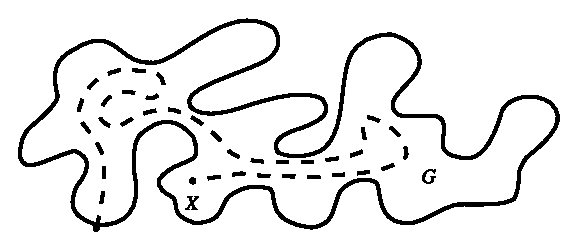
\includegraphics{figure/fig13.eps}
\end{figure}

The form of the solution is given directly by It\^o's formula (without
having recourse to the mean value property). If $u=u(X(t))$ satisfies
$\Delta u=0$ then by It\^o's formula
$$
du(X(t))=\langle \nabla u, dX\rangle.
$$

Therefore
$$
u(X(t))=u(X(0))+\int\limits^{t}_{0}\langle \nabla u(X(s)),dX(s)\rangle
$$\pageoriginale

Assuming $\nabla u$ to be bounded, we see that $u(X(t))$ is a
martingale. By the optional stopping theorem
$$
E(u(X(\tau))=u(X(0))=u(x).
$$

Thus It\^o's formula connects solutions of certain differential
equations with the hitting probabilities.







